\section{Assembling Multiple Insert Length Libraries}

\begin{note}
Like the previous examples, the data you will examine in this exercise is again
from Staphylococcus aureus which still has a genome of around 3MB. The reads are
Illumina paired end with an insert size of 170 bp and 350 bp.

You already downloaded the required reads from the SRA in previous exercises.
Specifically, the run data (SRR022863, SRR022852) from the SRA Study SRP001086.

\center{\url{http://www.ebi.ac.uk/ena/data/view/SRP001086}}
\end{note}

\begin{information}
The following exercise focuses on handing two insert length libraries with
velvet and the changes you have to look out for.
\end{information}

\begin{steps}
First move to the directory you made for this exercise, make a suitable named
directory for the exercise and check if all the files are in place:
\begin{lstlisting}
cd ~/NGS/velvet/part3
mkdir SRP001086
cd SRP001086
ln -s ~/NGS/Data/SRR022863_?.fastq.gz ./
ln -s ~/NGS/Data/SRR022852_?.fastq.gz ./
\end{lstlisting}

Now run \texttt{velveth} and \texttt{velvetg} using the appropriate command line
options by typing:
\begin{lstlisting}
time velveth run_25 25 -fmtAuto -create_binary -shortPaired -separate SRR022863_1.fastq.gz SRR022863_2.fastq.gz -shortPaired2 -separate SRR022852_1.fastq.gz SRR022852_2.fastq.gz
time velvetg run_25
\end{lstlisting}

The right thing to do is to run velvetg setting the cut-offs. To investigate
with R, as you did in the previous exercises, start up R and produce the
weighted histogram using the columns \texttt{short1\_cov} and
\texttt{short2\_cov} by typing:
\begin{lstlisting}[style=R]
R --no-save
library(plotrix) 
data <- read.table("run_25/stats.txt", header=TRUE) 
weighted.hist(data$short1_cov+data$short2_cov, data$lgth, breaks=0:70)
\end{lstlisting}

\begin{figure}[H]
\centering
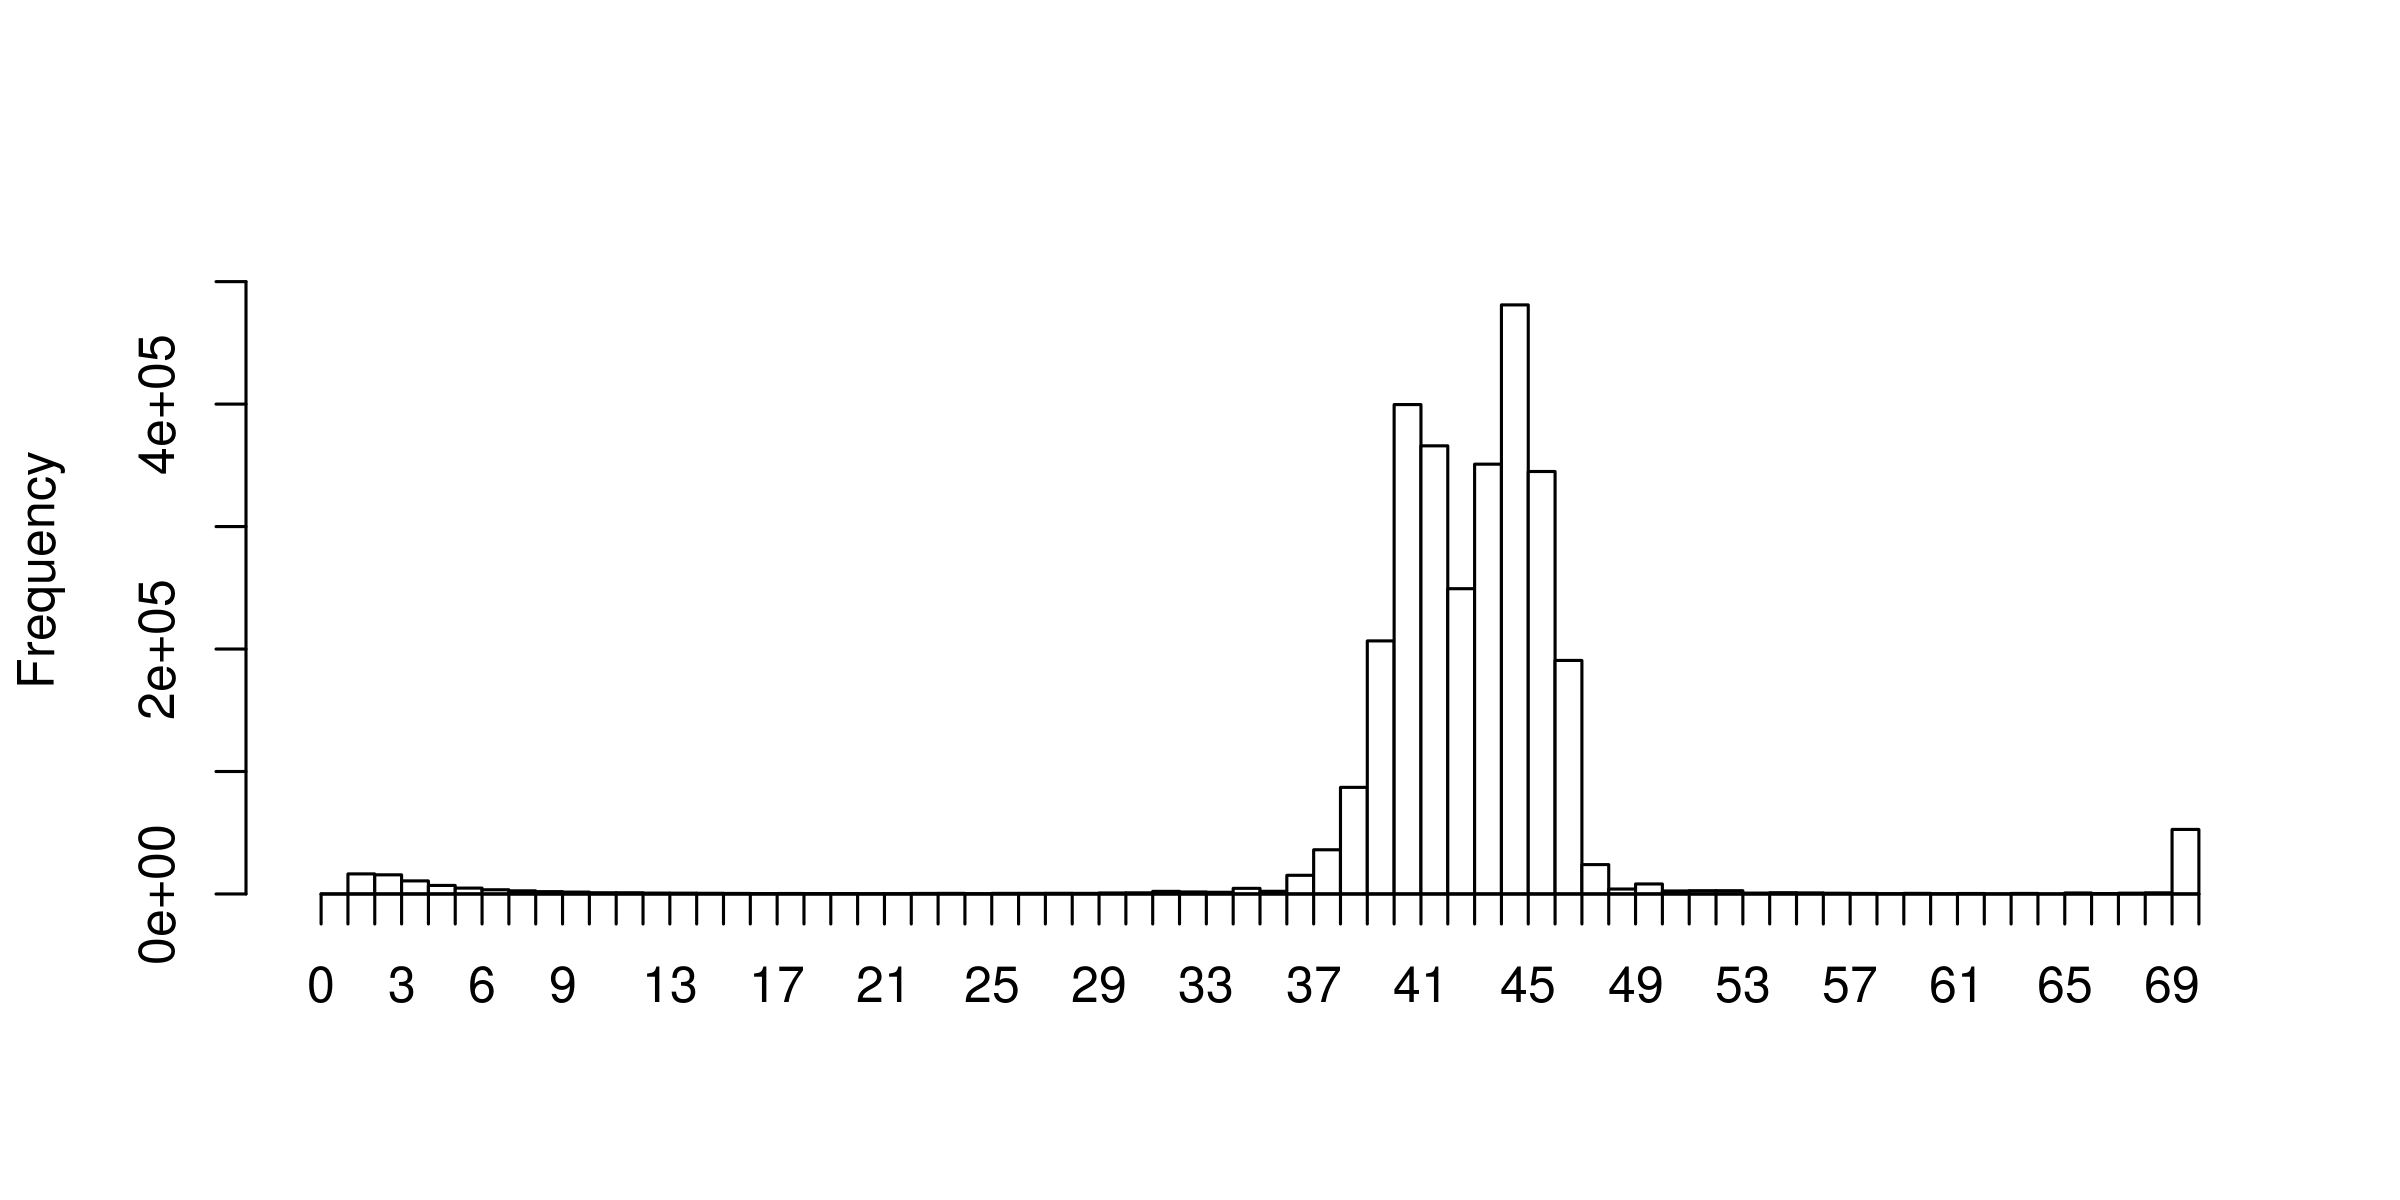
\includegraphics[width=0.8\textwidth]{de_novo/velvet/velvet_Rplot004.png}
\caption{\label{fig:velvet_Rplot004}}
\end{figure}

For me the histogram suggests a coverage cut-off of around 28
with an expected coverage of about 36. If you disagree, feel free to try
different settings, but first leave R before running \texttt{velvetg} with the coverage
parameters typing:
\begin{lstlisting}[style=R]
q()
\end{lstlisting}

\begin{lstlisting}
cp run_25/contigs.fa run_25/contigs.fa.0

time velvetg run_25 -cov_cutoff 28 
cp run_25/contigs.fa run_25/contigs.fa.1

time velvetg run_25 -cov_cutoff 28 -exp_cov 36 
cp run_25/contigs.fa run_25/contigs.fa.2

time velvetg run_25 -cov_cutoff 28 -exp_cov 36 -ins_length 170 -ins_length2 350
cp run_25/contigs.fa run_25/contigs.fa.3

gnx -min 100 -nx 25,50,75 run_25/contigs.fa*
\end{lstlisting}

\end{steps}

\begin{questions}
What was the best N50 you got?
\begin{answer}
62,741 bp
\end{answer}

How did the runtime/results compare to a run with a single paired-end library?
\begin{answer}
More memory, longer runtime, (in this case) similar results
\end{answer}

How many different libraries would you be able to run with this velvet version?
\begin{answer}
2 paired-end (or mate-pair) + one single end
\end{answer}

Would you be able to add a single-end library as well with this velvet version?
\begin{answer}
Yes
\end{answer}
\end{questions}


\begin{bonus}
Output an AMOS message file, convert it into an AMOS bank, update the
estimations for the insert size distributions and view the assembly with
Hawkeye.

\begin{lstlisting}
time velvetg run_25 -cov_cutoff 28 -exp_cov 36 -ins_length 170 -ins_length2 350 -amos_file yes -read_trkg yes
cp run_25/contigs.fa run_25/contigs.fa.4
gnx -min 100 -nx 25,50,75 run_25/contigs.fa.4

bank-transact -c -b run_25/velvet_asm.bnk -m run_25/velvet_asm.afg
asmQC -b run_25/velvet_asm.bnk -scaff -recompute -update -numsd 2
hawkeye run_25/velvet_asm.bnk
\end{lstlisting}

\begin{questions}
What are the mean and SD for the insert size distributions for the two libraries
used in the assembly?
\begin{answer}
Mean: 129; SD:31
Mean: 227; SD:19
\end{answer}
\end{questions}

\end{bonus}

% \begin{bonus}
% Find and download a different insert length library
% % TODO: \footnote affects the width of the shaded box - \renewcommand{\footnote}?
% \footnotemark[1]
% from the
% study SRP001086 and recompile velvet to allow the use of three insert length
% libraries. Maybe you could use the library you trimmed during previous
% exercises. You should be able to find these files here:
% \texttt{~/NGS/velvet/part2/SRX008042/SRR023408\_trim?.fastq}. If you don't still
% have these files, you can find a copy of them here:
% \texttt{~/NGS/Data/SRR023408\_trim?.fastq}.
% Use the fresh compiled Velvet version with the three (two provided and one
% downloaded library) to assemble the genome.
% \begin{questions}
% Does the extra library make any difference?
% \begin{answer}
% % TODO
% \end{answer}
% 
% How does the overall coverage change?
% \begin{answer}
% % TODO
% \end{answer}
% 
% Any other comments?
% \begin{answer}
% % TODO
% \end{answer}
% \end{questions}
% \footnotetext[1]{Paired insert
% lengths can be found on the NCBI SRA page in the library section (Nominal
% length) e.g. \url{http://www.ncbi.nlm.nih.gov/sra?term=SRR022866}}
% \end{bonus}
